\documentclass[11pt]{article}
\usepackage[margin=1in]{geometry}
\usepackage{amsmath,amssymb,mathtools}
\usepackage{booktabs}
\usepackage{enumitem}
\usepackage{siunitx}
\sisetup{group-separator={,},group-minimum-digits=3}

\title{\textbf{Quiz 2} \vspace{ 0.4cm }\\ECON 300: Labour Economics}
\author{Instructor: Muhebullah Karimzada}
\date{February 05,  2026}

\begin{document}
\maketitle

\vspace{1em}

\textbf{Instructions:}  
Choose the \textbf{best answer} for each question based on the following diagram.  

\vspace{1em}
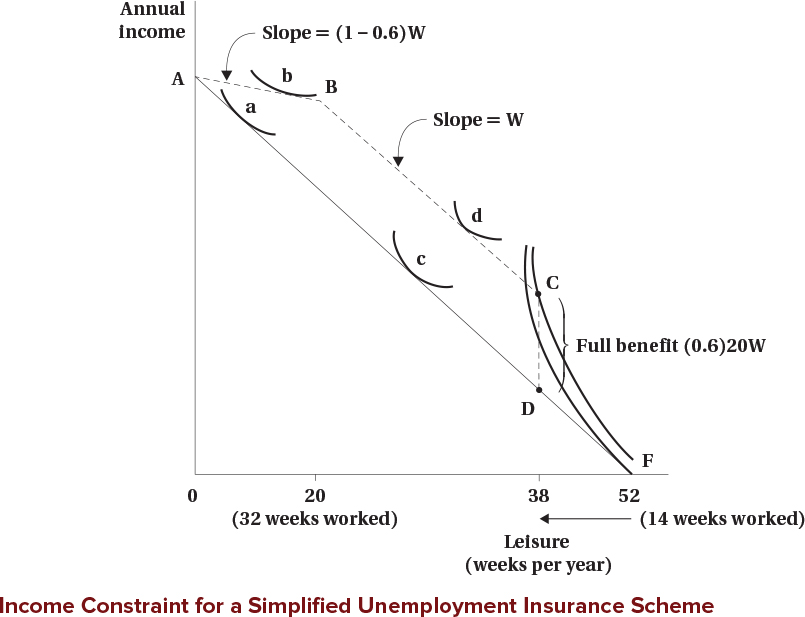
\includegraphics[width=0.61\linewidth]{ben54842_un0301}.

\begin{enumerate}

\item The segment of the budget constraint with slope \( (1 - 0.6)W \) represents:

\begin{enumerate}
\item The gross market wage  
\item The value of leisure  
\item The effective net wage while EI benefits are being reduced  
\item The reservation wage  
\end{enumerate}

\item The slope of the budget constraint between points \textbf{B} and \textbf{D} is equal to \( W \) because:

\begin{enumerate}
\item EI benefits are increasing in this region  
\item Benefits have been fully exhausted  
\item The worker is unemployed  
\item Leisure has zero opportunity cost  
\end{enumerate}

\item Point \textbf{A} in the diagram corresponds to:

\begin{enumerate}
\item Full-time work with no benefits  
\item Zero leisure and zero income  
\item Zero weeks worked with full EI benefits  
\item Partial employment with reduced benefits  
\end{enumerate}

\item Why is the budget constraint flatter between points \textbf{A} and \textbf{B} than between \textbf{B} and \textbf{D}?

\begin{enumerate}
\item The wage rate is lower in that range  
\item The worker faces payroll taxes  
\item EI benefits are clawed back as earnings increase  
\item Leisure is a normal good  
\end{enumerate}

\item The difference between the gross wage \( W \) and the effective wage \( (1 - 0.6)W \) reflects:

\begin{enumerate}
\item Employer payroll taxes  
\item Income taxes unrelated to EI  
\item The implicit tax created by the EI benefit reduction rate  
\item Minimum wage legislation  
\end{enumerate}

\item Which region of the budget constraint features the \textbf{highest effective marginal tax rate on earnings}?

\begin{enumerate}
\item Between points \textbf{B} and \textbf{D}  
\item Between points \textbf{D} and \textbf{F}  
\item Between points \textbf{A} and \textbf{B}  
\item At point \textbf{F}  
\end{enumerate}

\item Relative to a situation with no EI program, the EI scheme shown is most likely to:

\begin{enumerate}
\item Increase hours worked at all wage levels  
\item Reduce labour force participation for some individuals  
\item Increase the market wage paid by firms  
\item Eliminate income effects on labour supply  
\end{enumerate}

\item A worker who chooses a point like \textbf{B} rather than an interior point most likely does so because:

\begin{enumerate}
\item The worker’s marginal product is zero  
\item Leisure is inferior  
\item The worker faces a kink where work incentives change discretely  
\item The wage rate is higher at point \textbf{B}  
\end{enumerate}

\newpage
\item If the EI replacement rate were increased from 0.6 to 0.8, which of the following would occur?

\begin{enumerate}
\item The EI segment of the budget constraint would become steeper  
\item The effective net wage while on EI would increase  
\item The budget constraint while on EI would become flatter  
\item The gross wage would rise  
\end{enumerate}

\item From a policy perspective, the key efficiency concern illustrated by this diagram is that EI:

\begin{enumerate}
\item Reduces firms’ demand for labour  
\item Creates high effective marginal tax rates that discourage work  
\item Eliminates income risk entirely  
\item Raises long-run productivity  
\end{enumerate}

\end{enumerate}

\vfill
\textbf{End of Quiz}

\end{document}
